\chapter{Implementation}
\label{ch:impl}
\section{Environment Setup}
In this thesis, different techniques of recommendation algorithms have used to recommend recipes to users. The process of building recommendation models and evaluating those models requires high computational time and memory. The initial analysis is done on my personal machine but to achieve better efficiency and to reduce the execution time of the application, I chose to run it in the cloud environment.  In the current market, many cloud service providers are available such as Amazon Web Services (AWS), Microsoft Azure, Google Cloud Platform (GCP), IBM Cloud. To accelerate the execution performance of the analysis of this application, the Google Cloud Platform (GCP) is used. \\
\noindent GCP platform provides custom, configurable high-performance virtual machines with ease of application or scripts deployment via its User Interface (UI). There are three basic steps to run an application on a Virtual Machine (VM) on GCP. 
\subsection{Create GCP Account}
GCP account is linked with a user's Google account. One can enter into the GCP console dashboard by signing in with Google account. By default GCP creates a project for a user with the name `My First Project'. Users can create a new project here. I have created a project with the name `FeedMeRight'. As per \autoref{fig:gcp_dashboard} project id and project number have been created by GCP for the `FeedMeRight' project. 
\begin{figure}[H]
	\centering
	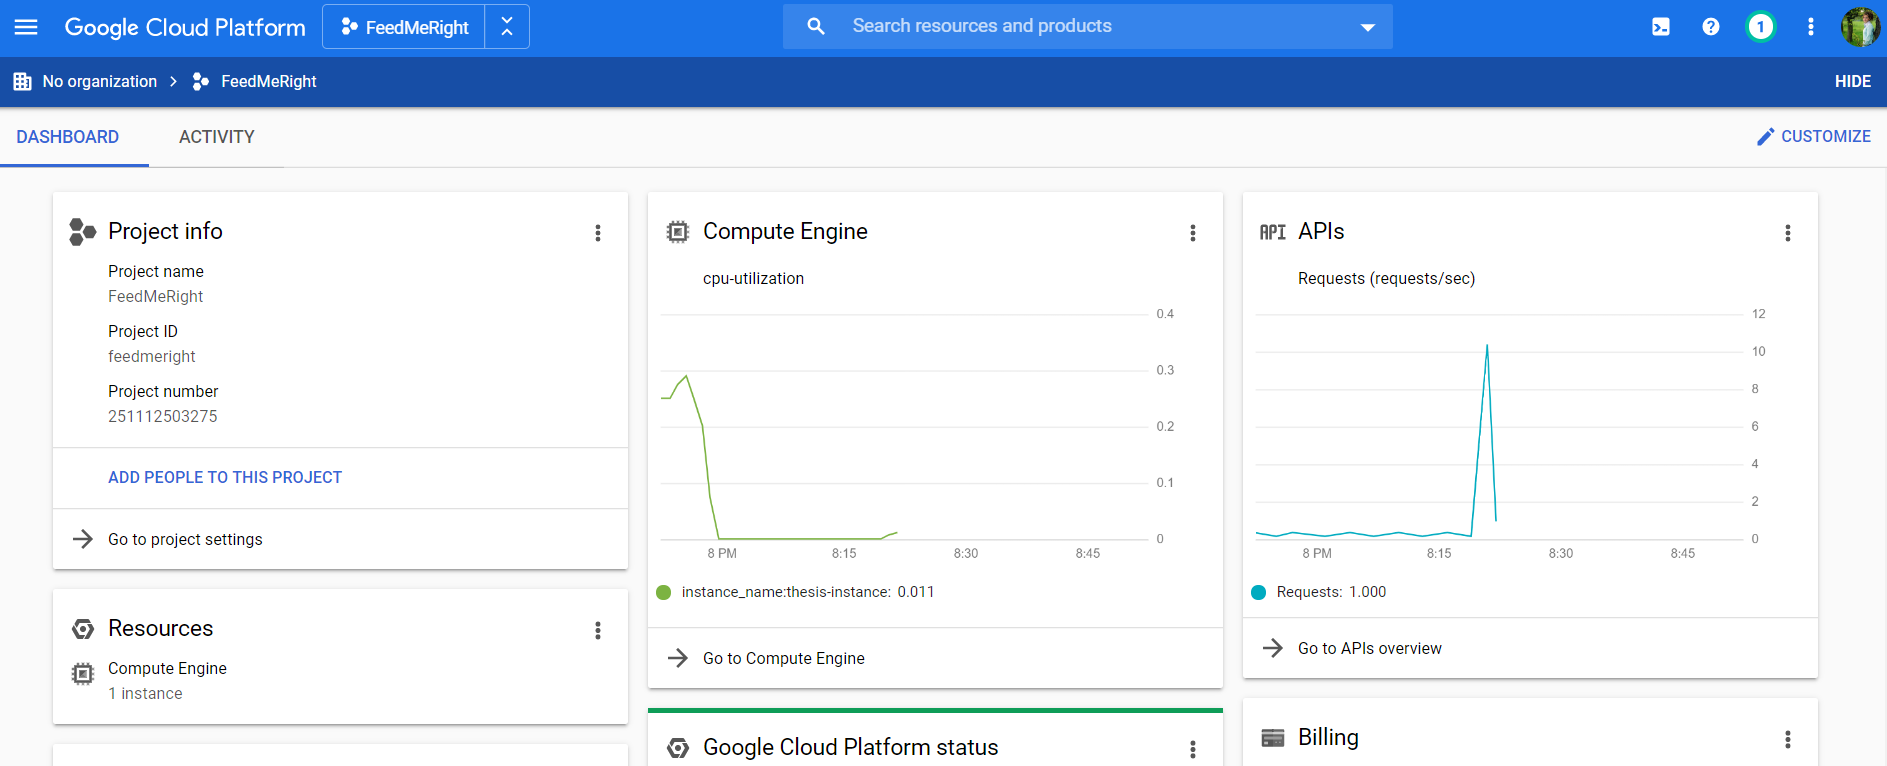
\includegraphics[width=1.0\linewidth]{GCP_Dashboard}
	\caption{GCP Dashboard}
	\label{fig:gcp_dashboard}
\end{figure}
  
\subsection{Virtual Machine (VM) on GCP}
Compute Engine lets you create and run virtual machines on Google Cloud Infrastructure. It helps to easily launch applications that require high computational capacity by offering scale, performance. Virtual machines are designed to be fast and to provide strong consistency of performance. 
\begin{figure}[H]
	\centering
	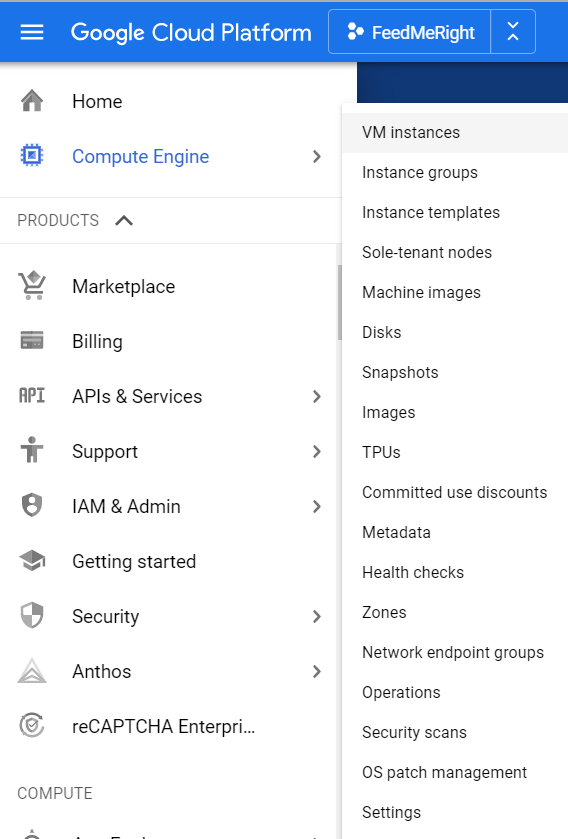
\includegraphics[width=0.50\linewidth]{vm_instance_option}
	\caption{GCP Service List}
	\label{fig:vm_instance_option}
\end{figure}

\noindent As per \autoref{fig:vm_instance_option}, with the help of `Compute Engine', virtual machine instance can be created. Created VM instance's settings can be customized. Configurations for `FeedMeRight' are used as shown in \autoref{fig:vm_configuration}.
\begin{figure}[H]
	\centering
	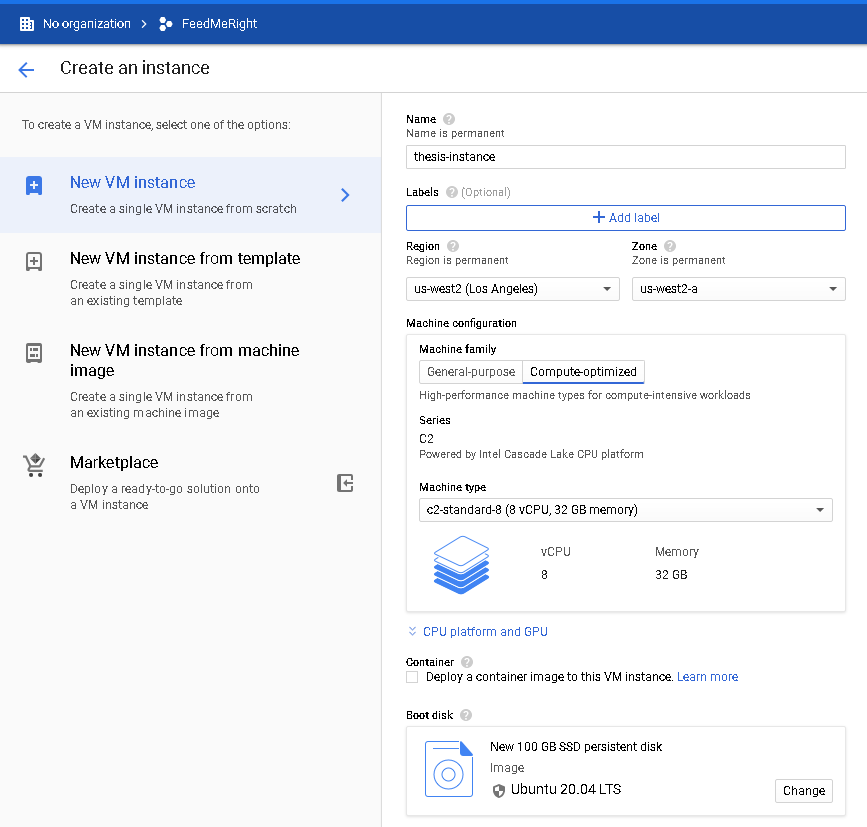
\includegraphics[width=1.0\linewidth]{vm_configuration}
	\caption{VM Configuration for FeedMeRight}
	\label{fig:vm_configuration}
\end{figure}

\subsection{Python Scripts Deployment}
After successful creation of VM instance, the application can be configured on this instance. To get all scripts created for `FeedMeRight' Git software has been used. Git is a version control system to keep track of changes in the source code. The source code for the project is stored on GitHub. GitHub is a cloud-based hosting service that lets you manage Git repositories. With the help of Git, we can pull all the source code stored in the cloud repository. To run the application, the installation of a set of libraries are required on VM. 

\begin{itemize}
\item \textbf{Numpy: } Numpy library provides support for large, multi-dimensional arrays and matrices. Also, it supports high-level mathematical functions.
\item \textbf{Pandas: } Pandas library provides data analysis and manipulation. It is a fast, powerful tool that offers data structure and operations for large files like CSV or TSV.
\item \textbf{Matplotlib: } Matplotlib is a plotting library for creating static, animated, and interactive visualizations in Python. It is based on Numpy and Pandas libraries.
\item \textbf{Scikit-learn: } Scikit-learn is a machine learning library that provides various machine learning algorithms.
\item \textbf{NLTK: } NLTK is a toolkit to process human's natural language.
\item \textbf{SciPy: } SciPy library is used for scientific and technical computing. It builds on Numpy. 
\item \textbf{Anaconda: } Anaconda is a python package management and deployment software that makes it easy for developers to create different virtual environments.  
\item \textbf{Jupyter NoteBook: } Jupyter Notebook is a web application that can be used to create and share documents that have live code in it. It provides User Interface that makes easy interaction and visualization of results. 
\item \textbf{PyCharm: } PyCharm is an Integrated Development Environment (IDE) used for python programming language. 
\end{itemize}  